\begin{frame}[allowframebreaks]{Clustering}
\begin{columns}
    \begin{column}{0.45\textwidth}
        A set of methods for finding  subgroups within the dataset. 
        \vspace{0.8em}
        \begin{itemize}
            \setlength{\itemsep}{0.5em}
            \item Observations should share  common characteristics within the  same group, but differ across  groups.
            \item Groupings are determined from  attributes of the data itself —  differs from classification.
        \end{itemize}
    \end{column}
    \begin{column}{0.55\textwidth}
        \begin{figure}
            \centering
            \fetchconvertimage{https://miro.medium.com/v2/resize:fit:720/format:webp/0*Jwm3mV92c3qRhqEl.}{images/clustering-example.png}{width=0.95\textwidth,keepaspectratio}
            \caption{Taking a 2 dimensional dataset and separating it into 3 distinct clusters. [\href{https://medium.com/square-corner-blog/so-you-have-some-clusters-now-what-abfd297a575b}{Source}]}
        \end{figure}
    \end{column}
\end{columns}

\framebreak

\begin{algorithm}[H]
\caption{Generic Clustering Algorithm}

\KwIn{Dataset $D = \{x_1, x_2, \dots, x_n\}$, number of clusters $k$}
\KwOut{Cluster assignments for each data point}

\vspace{0.5em}
\textbf{Initialization:} Randomly initialize $k$ cluster centroids or seeds\;

\vspace{0.5em}
\Repeat{convergence or maximum iterations reached}{
    \vspace{0.3em}
    \textbf{Assignment Step:} Assign each data point $x_i$ to the nearest cluster based on a distance metric\;
    
    \vspace{0.3em}
    \textbf{Update Step:} Recompute cluster centroids using current assignments\;
}

\vspace{0.5em}
\Return Final cluster assignments\;
\vspace{0.8em}

\end{algorithm}
\end{frame}

\begin{frame}[allowframebreaks]{Clustering Vs Classification}
\begin{figure}
    \centering
    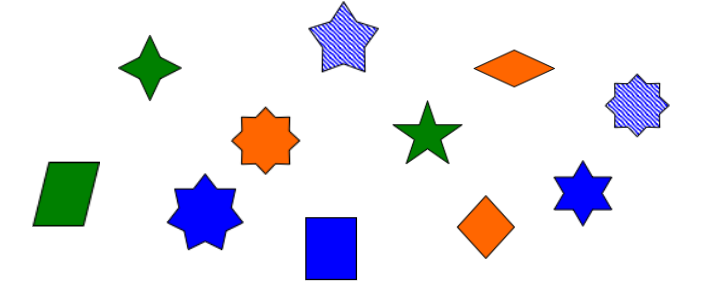
\includegraphics[width=0.8\textwidth,keepaspectratio]{images/sample-clustering-classification.png}
    \caption{Sample data points.}
\end{figure}

\framebreak

\begin{columns}
    \begin{column}{0.5\textwidth}
        \textbf{Classification}
        \begin{itemize}
            \item Labels available
            \item Assigning to known classes
            \item Supervised
        \end{itemize}
        \vspace{1.8em}
        \begin{figure}
            \centering
            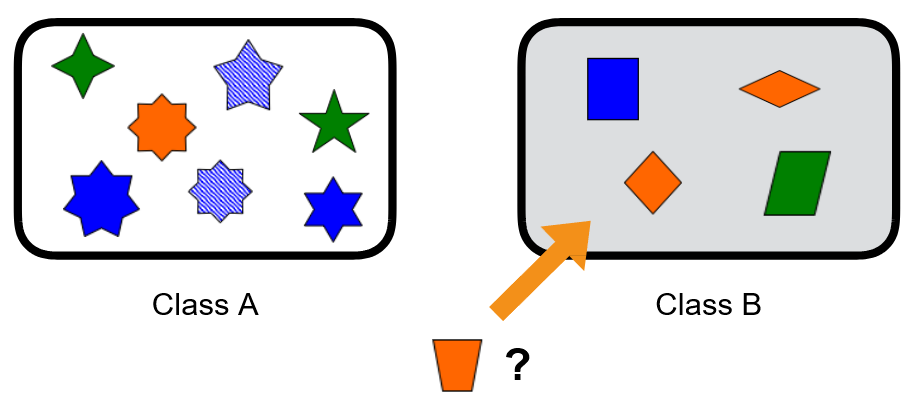
\includegraphics[width=1\textwidth,keepaspectratio]{images/sample-result-classification.png}
            \caption{Classification result.}
        \end{figure}
    \end{column}
    \begin{column}{0.5\textwidth}
        \textbf{Clustering}
        \begin{itemize}
            \item No labels
            \item Grouping based on similarity
            \item Unsupervised
        \end{itemize}
        \vspace{1.8em}
        \begin{figure}
            \centering
            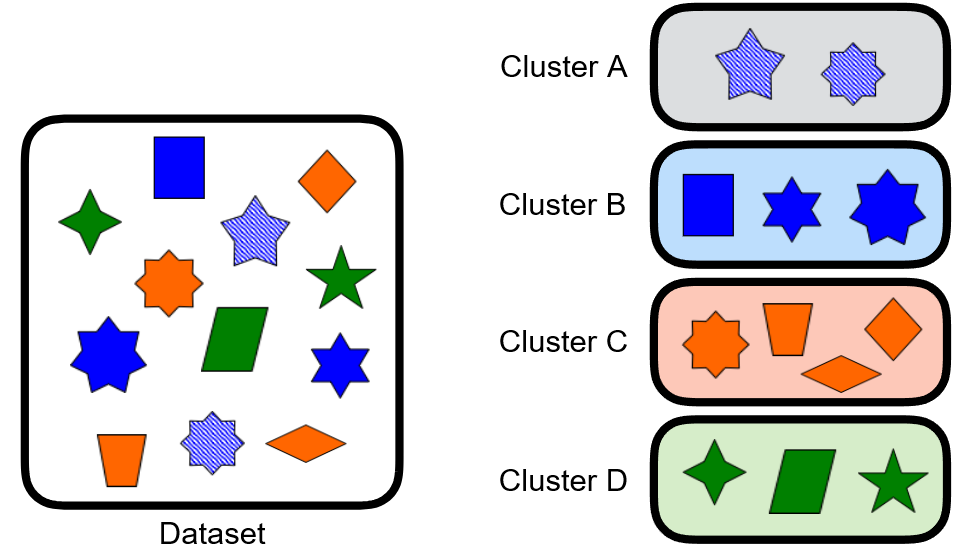
\includegraphics[width=1\textwidth,keepaspectratio]{images/sample-result-clustering.png}
            \caption{Clustering result.}
        \end{figure}
    \end{column}
\end{columns}
\end{frame}

\begin{frame}[allowframebreaks]{Clustering: Types}
    \begin{itemize}
        \item \textbf{Centroid-Based Clustering}: Groups data points based on their proximity to a central point, such as K-means or K-medoids.
        \item \textbf{Hierarchical Clustering}: Builds a hierarchy of clusters using either agglomerative (bottom-up) or divisive (top-down) approaches.
        \item \textbf{Model-Based Clustering}:
        \begin{itemize}
            \item Each cluster is represented by a parametric distribution.
            \item Dataset is a mixture of distributions.
            \item Assumes a probabilistic model for the data and uses statistical methods to identify clusters, such as Gaussian Mixture Models (GMM).
        \end{itemize}
        \item \textbf{Hard Clustering}: 
        \begin{itemize}
            \item Each data point is assigned exclusively to exactly one cluster.
            \item \textbf{Example algorithms}: K-means, Hierarchical clustering.
            \item \textbf{interpretation}: No ambiguity — clusters are crisp and non-overlapping.
        \end{itemize}
        \item \textbf{Soft/Fuzzy Clustering}: 
        \begin{itemize}
            \item Each data point can belong to multiple clusters simultaneously with varying degrees of membership (probabilities or weights).
            \item \textbf{Example algorithms}: Gaussian Mixture Models (GMM), Fuzzy C-means.
            \item \textbf{interpretation}: Reflects uncertainty or mixed membership — clusters can overlap.
        \end{itemize}
    \end{itemize}
\end{frame}